%% LyX 2.4.4 created this file.  For more info, see https://www.lyx.org/.
%% Do not edit unless you really know what you are doing.
\documentclass[english,t]{beamer}
\usepackage{mathptmx}
\usepackage[T1]{fontenc}
\usepackage[latin9]{inputenc}
\usepackage{units}
\usepackage{amssymb}
\usepackage{cancel}

\makeatletter
%%%%%%%%%%%%%%%%%%%%%%%%%%%%%% Textclass specific LaTeX commands.
% this default might be overridden by plain title style
\newcommand\makebeamertitle{\frame{\maketitle}}%
% (ERT) argument for the TOC
\AtBeginDocument{%
  \let\origtableofcontents=\tableofcontents
  \def\tableofcontents{\@ifnextchar[{\origtableofcontents}{\gobbletableofcontents}}
  \def\gobbletableofcontents#1{\origtableofcontents}
}

%%%%%%%%%%%%%%%%%%%%%%%%%%%%%% User specified LaTeX commands.
\usetheme{Warsaw}
% or ...

\setbeamercovered{transparent}
% or whatever (possibly just delete it)
\setbeamercovered{invisible} %makes overlays invisible

%gets rid of navigation symbols
\setbeamertemplate{navigation symbols}{}

%\usepackage{hyperref}
%\usepackage[usenames,dvipsnames,table]{xcolor} %adds additional color options
\definecolor{links}{HTML}{2A1B81}
%\hypersetup{colorlinks,linkcolor=blue,urlcolor=links}

\usepackage{multicol}

\usepackage{hyperref}

\usepackage{tikz}
\usetikzlibrary{calc}
\usetikzlibrary{plotmarks}
\usetikzlibrary{shapes}
\usepackage{pgfplots} %\usepackage{pgfplots, pgfplotstable}
\pgfplotsset{compat=newest}
\usepackage{filecontents}  %allows in file data
\usepgfplotslibrary{statistics} %allows histogram stuff

\usepackage{forest} %%for tree diagram

\usepackage{calc}
\usepackage[nomessages]{fp}

\usepackage[super]{nth} %easy 1st, 2nd, etc

%\usepackage{advdate}    % Advancing/saving dates
\usepackage{datetime}   % Dates formatting
%\usepackage{datenumber} % Counters for dates

\usepackage[super]{nth}

\usepackage{etex}

\usepackage{fancybox}

%%table colors
%\usepackage[table]{xcolor}
\usepackage{colortbl}

\usepackage[outline]{contour}  %allows text halos

\usepackage{epsdice} %%dice font
\usepackage[misc]{ifsym}
\newfont\dice{dice3d} %%3d dice font

\contourlength{1pt} %sets halo width
%%example: \node at (0.75,0.5) {\contour{white}{\Large Text!}};
%%example:  \node [fill=white,inner sep=1pt] at (2.25,0.5) {\Large 			Text!};
%%example:  \node [fill=white,rounded corners=2pt,inner sep=1pt] at 			(3.75,0.5) {\Large Text!};

%%%%%%%%%%%%%%%%%%%%%%%%%%%
\def\formatdateny{\csname noyear\languagename\expandafter\endcsname\formatdate}
\def\noyearenglish#1, \the\@year{#1}
\let\noyearamerican\noyearenglish
\let\noyearbritish\noyearenglish

%%allows uncover with forest diagrams
\tikzset{
    invisible/.style={opacity=0,text opacity=0},
    visible on/.style={alt=#1{}{invisible}},
    alt/.code args={<#1>#2#3}{%
      \alt<#1>{\pgfkeysalso{#2}}{\pgfkeysalso{#3}} % \pgfkeysalso doesn't change the path
    },
}
\forestset{
  visible on/.style={
    for tree={
      /tikz/visible on={#1},
      edge={/tikz/visible on={#1}}}}}

%%%redefines column alignment to match vertically
%\define@key{beamerframe}{t}[true]{% top
  %\beamer@frametopskip=.2cm plus .5\paperheight\relax%
  %\beamer@framebottomskip=0pt plus 1fill\relax%
 % \beamer@frametopskipautobreak=\beamer@frametopskip\relax%
  %\beamer@framebottomskipautobreak=\beamer@framebottomskip\relax%
  %\def\beamer@initfirstlineunskip{}%
%}

%%provides pdf with 4 slides per page; don't forget to add 'handout' to remove overlays
%\usepackage{pgfpages}
%\pgfpagesuselayout{4 on 1}[a4paper, landscape, border shrink=7mm]
%\pgfpageslogicalpageoptions{1}{border code=\pgfusepath{stroke}}
%\pgfpageslogicalpageoptions{2}{border code=\pgfusepath{stroke}}
%\pgfpageslogicalpageoptions{3}{border code=\pgfusepath{stroke}}
%\pgfpageslogicalpageoptions{4}{border code=\pgfusepath{stroke}}
%%%Don't forget to add 'handout'

\makeatother

\usepackage{babel}
\begin{document}
\newcommand{\gauss}[2]{1/(#2*sqrt(2*pi))*exp(-((x-#1)^2)/(2*#2^2))}

\newcommand{\xmax}{2000}
\newcommand{\xmin}{0}
\newcommand{\xstep}{0} %must be xmin+n
\newcommand{\ymax}{500}
\newcommand{\ymin}{0}
\newcommand{\ystep}{0} %must be ymin+n

\newcounter{countEx} \setcounter{countEx}{0}
\newcounter{countProb} \setcounter{countProb}{0}
\resetcounteronoverlays{countEx} \resetcounteronoverlays{countProb}

\newcommand{\ex}[3]{
	\addtocounter{countEx}{1}
	\only<#1-#2>{\begin{exampleblock} {Example \chNum.\secNum.\arabic{countEx}.} #3	\end{exampleblock}}
}

\newcommand{\prob}[4]{
	\addtocounter{countProb}{1}
	\only<#1-#2>{\begin{exampleblock} {Problem  \chNum.\secNum.\arabic{countProb}.\,#3} #4	\end{exampleblock}}
}

\newcommand{\yline}[4]{
	(#2 - #4)/(#1 - #3)*(x - #1) + #2
}

\beamerdefaultoverlayspecification{<+->}

%%%%Chapter and Section numbers%%%%%
\newcommand{\chNum}{4}
\newcommand{\secNum}{4}
\newcommand{\secTitle}{The Normal Distribution}
\date{\formatdate{5}{11}{2014}}

\title[Section \chNum.\secNum: \secTitle]{Section \chNum.\secNum: \secTitle}

\subtitle{Finite Mathematics~~MTH 107~~Fall 2014}

\author{Dr.\,James Ashe}

\titlegraphic{\includegraphics[height=2.75cm]{/home/jim/JamesAshe/MHU/images/MarsHilUniversityLogo-Virtical.png}}

\institute{Mars Hill University}

\makebeamertitle 

%%True false command
\newcommand{\T}{\textcolor{green}{\contour{black}{T}}}
\newcommand{\F}{\textcolor{red}{\contour{black}{F}}}
\newcommand{\uT}[2]{\uncover<#1-#2>{\T}}
\newcommand{\uF}[2]{\uncover<#1-#2>{\F}}

%tkiz ball item 
\newcommand*\circled[1]{\tikz[baseline=(char.base)]
	{\node[circle,ball color=green!50!black!100, shade,   color=white,inner sep=1.2pt] (char) {\tiny #1};
	}
}
\begin{frame}{Discrete vs Continuous Variables}

\begin{columns}


\column{5.5cm}
\begin{itemize}
\item []\textbf{Discrete}
\item [ex.] Number of students in class
\item [ex.] Integers:
\item []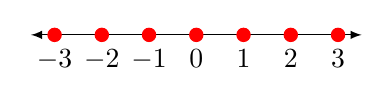
\begin{tikzpicture}[scale=.6] 
	%\draw[very thick] (1,0) -- (2,0); 
	\draw[latex-latex] (-3.5,0) -- (3.5,0); 
	\foreach \x in  {-3,-2,-1,0,1,2,3} 
	\draw[shift={(\x,0)},color=black] (0pt,3pt) -- (0pt,-3pt); 
	\foreach \x in {-3,-2,-1,0,1,2,3} 
	\draw[shift={(\x,0)},color=black] (0pt,0pt) -- (0pt,-3pt) node[below]  {$\x$};
	\path [draw=red, fill=red] (1,0) circle (4pt);
	\path [draw=red, fill=red] (2,0) circle (4pt);
	\path [draw=red, fill=red] (3,0) circle (4pt);
	\path [draw=red, fill=red] (0,0) circle (4pt);
	\path [draw=red, fill=red] (-1,0) circle (4pt);
	\path [draw=red, fill=red] (-2,0) circle (4pt);
	\path [draw=red, fill=red] (-3,0) circle (4pt);
\end{tikzpicture}
\item [ex.] Votes for a canidate
\item [ex.] Money: $1$, $.25$, $.10$, $.05$, $.01$
\end{itemize}

\column{5.5cm}
\begin{itemize}
\item []\textbf{Continuous}
\item [ex.] The real numbers
\item [ex.] $-\nicefrac{1}{2}<x\leq3$
\item []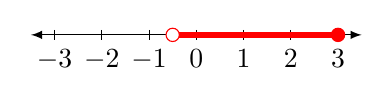
\begin{tikzpicture}[scale=.6] 
	\draw[latex-latex] (-3.5,0) -- (3.5,0); 
	\foreach \x in  {-3,-2,-1,0,1,2,3} 
	\draw[shift={(\x,0)},color=black] (0pt,3pt) -- (0pt,-3pt); 
	\foreach \x in {-3,-2,-1,0,1,2,3} 
	\draw[shift={(\x,0)},color=black] (0pt,0pt) -- (0pt,-3pt) node[below]  {$\x$};
	\draw[red,line width=.75mm] (-0.5,0) -- (3,0); 
	\path [draw=red, fill=white] (-0.5,0) circle (4pt);
	\path [draw=red, fill=red] (3,0) circle (4pt);
\end{tikzpicture}
\item [ex.] height, weight, time, etc.
\end{itemize}
\end{columns}
\end{frame}

\begin{frame}{Heights of Men}

\begin{columns}


\column{4cm}
\begin{itemize}
\item []The heights of $10,000$ randomly selected men.

\begin{itemize}
\item <2->$n=10,000$
\item <3->$\bar{x}=70$ inches
\item <4->$s=3$ inches
\end{itemize}
\end{itemize}

\column{6cm}

\textbf{Histogram}

\begin{center}
\only<5-5>{\begin{tikzpicture}[scale=.75]
\begin{axis}[     ybar,     ymin=0 ]
\addplot+[hist={bins=5}] table [y index=0] {men_height.csv};
\end{axis} 
\end{tikzpicture} 
\par\end{center}
\begin{itemize}
\item $5$ groups
\end{itemize}
\begin{center}
}\only<6-6>{\begin{tikzpicture}[scale=.75]
\begin{axis}[     ybar,     ymin=0 ]
\addplot+[hist={bins=10}] table [y index=0] {men_height.csv};
\end{axis} 
\end{tikzpicture} 
\par\end{center}
\begin{itemize}
\item $10$ groups
\end{itemize}
\begin{center}
}\only<7-7>{\begin{tikzpicture}[scale=.75]
\begin{axis}[     ybar,     ymin=0 ]
\addplot+[hist={bins=25}] table [y index=0] {men_height.csv};
\end{axis} 
\end{tikzpicture} 
\par\end{center}
\begin{itemize}
\item $25$ groups
\end{itemize}
\begin{center}
}\only<8-8>{\begin{tikzpicture}[scale=.75]
\begin{axis}[     ybar,     ymin=0 ]
\addplot+[hist={bins=50}] table [y index=0] {men_height.csv};
\end{axis} 
\end{tikzpicture} 
\par\end{center}
\begin{itemize}
\item $50$ groups
\end{itemize}
\begin{center}
}\only<9-9>{\begin{tikzpicture}[scale=.75]
\begin{axis}[     ybar,     ymin=0 ]
\addplot+[hist={bins=100}] table [y index=0] {men_height.csv};
\end{axis} 
\end{tikzpicture} 
\par\end{center}
\begin{itemize}
\item $100$ groups
\end{itemize}
\begin{center}
}
\par\end{center}

\end{columns}
\end{frame}

\begin{frame}{Standard Normal Distribution}

\begin{columns}


\column{4cm}
\begin{itemize}
\item []Sums of 10,000 randomly generated numbers.

\begin{itemize}
\item <2->$n=10,000$
\item <3->$\bar{x}=0$
\item <4->$s=1$ 
\end{itemize}
\end{itemize}

\column{6cm}

\textbf{Histogram}

\begin{center}
\only<5-5>{\begin{tikzpicture}[scale=.75]
\begin{axis}[     ybar,     ymin=0 ]
\addplot+[hist={bins=5}] table [y index=0] {10000rand.csv};
\end{axis} 
\end{tikzpicture} 
\par\end{center}
\begin{itemize}
\item $5$ groups
\end{itemize}
\begin{center}
}\only<6-6>{\begin{tikzpicture}[scale=.75]
\begin{axis}[     ybar,     ymin=0 ]
\addplot+[hist={bins=10}] table [y index=0] {10000rand.csv};
\end{axis} 
\end{tikzpicture} 
\par\end{center}
\begin{itemize}
\item $10$ groups
\end{itemize}
\begin{center}
}\only<7-7>{\begin{tikzpicture}[scale=.75]
\begin{axis}[     ybar,     ymin=0 ]
\addplot+[hist={bins=25}] table [y index=0] {10000rand.csv};
\end{axis} 
\end{tikzpicture} 
\par\end{center}
\begin{itemize}
\item $25$ groups
\end{itemize}
\begin{center}
}\only<8-8>{\begin{tikzpicture}[scale=.75]
\begin{axis}[     ybar,     ymin=0 ]
\addplot+[hist={bins=50}] table [y index=0] {10000rand.csv};
\end{axis} 
\end{tikzpicture} 
\par\end{center}
\begin{itemize}
\item $50$ groups
\end{itemize}
\begin{center}
}\only<9-9>{\begin{tikzpicture}[scale=.75]
\begin{axis}[     ybar,     ymin=0 ]
\addplot+[hist={bins=100}] table [y index=0] {10000rand.csv};
\end{axis} 
\end{tikzpicture} 
\par\end{center}
\begin{itemize}
\item $100$ groups
\end{itemize}
\begin{center}
}
\par\end{center}

\end{columns}
\end{frame}

\begin{frame}{Normal Distribution}

\begin{columns}


\column{10cm}

\vspace{0cm}\begin{tikzpicture} 
\begin{axis}[ 
	no markers, 
	domain=0:10, 
	%samples=100, 
	axis lines*=left, 
	xlabel=Standard deviations, 
	ylabel=Frequency, 
	%height=6cm, 
	%width=10cm, 
	xtick={-3, -2, -1, 0, 1, 2, 3}, 
	%ytick=empty, 
	enlargelimits=false, 
	clip=false, 
	axis on top, 
	%grid = major
	] 
	\addplot [fill=cyan!20, draw, very thick, smooth, domain=-3:3] {\gauss{0}{1}} \closedcycle; 
	%\addplot [fill=orange!20, draw=none, domain=-3:-2] {\gauss{0}{1}} \closedcycle; 
	%\addplot [fill=orange!20, draw=none, domain=2:3] {\gauss{0}{1}} \closedcycle; 
	%\addplot [fill=blue!20, draw=none, domain=-2:-1] {\gauss{0}{1}} \closedcycle; 
	%\addplot [fill=blue!20, draw=none, domain=1:2] {\gauss{0}{1}} \closedcycle; 
	%\addplot[<->] coordinates {(-1,0.4) (1,0.4)}; 
	%\addplot[<->] coordinates {(-2,0.3) (2,0.3)}; 
	%\addplot[<->] coordinates {(-3,0.2) (3,0.2)}; 
	%\node[coordinate, pin={68.2%}] at (axis cs: 0, 0.4){}; 
	%\node[coordinate, pin={95%}] at (axis cs: 0, 0.3){}; 
	%\node[coordinate, pin={99.7%}] at (axis cs: 0, 0.2){}; 
	%\node[coordinate, pin={34.1%}] at (axis cs: -0.5, 0){}; 
	%\node[coordinate, pin={34.1%}] at (axis cs: 0.5, 0){}; 
	%\node[coordinate, pin={13.6%}] at (axis cs: 1.5, 0){}; 
	%\node[coordinate, pin={13.6%}] at (axis cs: -1.5, 0){}; 
	%\node[coordinate, pin={2.1%}] at (axis cs: 2.5, 0){}; 
	%\node[coordinate, pin={2.1%}] at (axis cs: -2.5, 0){}; 
	\end{axis} 
\end{tikzpicture}

\column{2cm}
\begin{itemize}
\item <2->[$\bar{x}=0$]
\item <3->[$s=1$]
\end{itemize}
\end{columns}
\end{frame}

\begin{frame}{Normal Distribution}

\begin{columns}


\column{10cm}

\vspace{0cm}\begin{tikzpicture} 
\begin{axis}[ 
	no markers, 
	domain=0:10, 
	%samples=100, 
	axis lines*=left, 
	xlabel=Standard deviations, 
	ylabel=Frequency, 
	%height=6cm, 
	%width=10cm, 
	%xtick={-3, -2, -1, 0, 1, 2, 3}, 
	%ytick=empty, 
	enlargelimits=false, 
	clip=false, 
	axis on top, 
	%grid = major
	] 
	\addplot [fill=cyan!20, draw, very thick, smooth, domain=7:13] {\gauss{10}{1}} \closedcycle; 
	%\addplot [fill=orange!20, draw=none, domain=-3:-2] {\gauss{0}{1}} \closedcycle; 
	%\addplot [fill=orange!20, draw=none, domain=2:3] {\gauss{0}{1}} \closedcycle; 
	%\addplot [fill=blue!20, draw=none, domain=-2:-1] {\gauss{0}{1}} \closedcycle; 
	%\addplot [fill=blue!20, draw=none, domain=1:2] {\gauss{0}{1}} \closedcycle; 
	%\addplot[<->] coordinates {(-1,0.4) (1,0.4)}; 
	%\addplot[<->] coordinates {(-2,0.3) (2,0.3)}; 
	%\addplot[<->] coordinates {(-3,0.2) (3,0.2)}; 
	%\node[coordinate, pin={68.2%}] at (axis cs: 0, 0.4){}; 
	%\node[coordinate, pin={95%}] at (axis cs: 0, 0.3){}; 
	%\node[coordinate, pin={99.7%}] at (axis cs: 0, 0.2){}; 
	%\node[coordinate, pin={34.1%}] at (axis cs: -0.5, 0){}; 
	%\node[coordinate, pin={34.1%}] at (axis cs: 0.5, 0){}; 
	%\node[coordinate, pin={13.6%}] at (axis cs: 1.5, 0){}; 
	%\node[coordinate, pin={13.6%}] at (axis cs: -1.5, 0){}; 
	%\node[coordinate, pin={2.1%}] at (axis cs: 2.5, 0){}; 
	%\node[coordinate, pin={2.1%}] at (axis cs: -2.5, 0){}; 
	\end{axis} 
\end{tikzpicture}

\column{2cm}
\begin{itemize}
\item <2->[$\bar{x}=10$]
\item <3->[$s=1$]
\end{itemize}
\end{columns}
\end{frame}

\begin{frame}{Normal Distribution}

\begin{columns}


\column{10cm}

\vspace{0cm}\begin{tikzpicture} 
\begin{axis}[ 
	no markers, 
	domain=0:10, 
	%samples=100, 
	axis lines*=left, 
	xlabel=Standard deviations, 
	ylabel=Frequency, 
	%height=6cm, 
	%width=10cm, 
	%xtick={-3, -2, -1, 0, 1, 2, 3}, 
	%ytick=empty, 
	enlargelimits=false, 
	clip=false, 
	axis on top, 
	%grid = major
	] 
	\addplot [fill=cyan!20, draw, very thick, smooth, domain=7:13] {\gauss{10}{.5}} \closedcycle; 
	%\addplot [fill=orange!20, draw=none, domain=-3:-2] {\gauss{0}{1}} \closedcycle; 
	%\addplot [fill=orange!20, draw=none, domain=2:3] {\gauss{0}{1}} \closedcycle; 
	%\addplot [fill=blue!20, draw=none, domain=-2:-1] {\gauss{0}{1}} \closedcycle; 
	%\addplot [fill=blue!20, draw=none, domain=1:2] {\gauss{0}{1}} \closedcycle; 
	%\addplot[<->] coordinates {(-1,0.4) (1,0.4)}; 
	%\addplot[<->] coordinates {(-2,0.3) (2,0.3)}; 
	%\addplot[<->] coordinates {(-3,0.2) (3,0.2)}; 
	%\node[coordinate, pin={68.2%}] at (axis cs: 0, 0.4){}; 
	%\node[coordinate, pin={95%}] at (axis cs: 0, 0.3){}; 
	%\node[coordinate, pin={99.7%}] at (axis cs: 0, 0.2){}; 
	%\node[coordinate, pin={34.1%}] at (axis cs: -0.5, 0){}; 
	%\node[coordinate, pin={34.1%}] at (axis cs: 0.5, 0){}; 
	%\node[coordinate, pin={13.6%}] at (axis cs: 1.5, 0){}; 
	%\node[coordinate, pin={13.6%}] at (axis cs: -1.5, 0){}; 
	%\node[coordinate, pin={2.1%}] at (axis cs: 2.5, 0){}; 
	%\node[coordinate, pin={2.1%}] at (axis cs: -2.5, 0){}; 
	\end{axis} 
\end{tikzpicture}

\column{2cm}
\begin{itemize}
\item <2->[$\bar{x}=10$]
\item <3->[$s=.5$]
\end{itemize}
\end{columns}
\end{frame}

\begin{frame}{Normal Distribution}

\begin{columns}


\column{10cm}

\vspace{0cm}\begin{tikzpicture} 
\begin{axis}[ 
	no markers, 
	domain=0:10, 
	%samples=100, 
	axis lines*=left, 
	xlabel=Standard deviations, 
	ylabel=Frequency, 
	%height=6cm, 
	%width=10cm, 
	%xtick={-3, -2, -1, 0, 1, 2, 3}, 
	%ytick=empty, 
	enlargelimits=false, 
	clip=false, 
	axis on top, 
	%grid = major
	] 
	\addplot [fill=cyan!20, draw, very thick, smooth, domain=-2:22] {\gauss{10}{4}} \closedcycle; 
	%\addplot [fill=orange!20, draw=none, domain=-3:-2] {\gauss{0}{1}} \closedcycle; 
	%\addplot [fill=orange!20, draw=none, domain=2:3] {\gauss{0}{1}} \closedcycle; 
	%\addplot [fill=blue!20, draw=none, domain=-2:-1] {\gauss{0}{1}} \closedcycle; 
	%\addplot [fill=blue!20, draw=none, domain=1:2] {\gauss{0}{1}} \closedcycle; 
	%\addplot[<->] coordinates {(-1,0.4) (1,0.4)}; 
	%\addplot[<->] coordinates {(-2,0.3) (2,0.3)}; 
	%\addplot[<->] coordinates {(-3,0.2) (3,0.2)}; 
	%\node[coordinate, pin={68.2%}] at (axis cs: 0, 0.4){}; 
	%\node[coordinate, pin={95%}] at (axis cs: 0, 0.3){}; 
	%\node[coordinate, pin={99.7%}] at (axis cs: 0, 0.2){}; 
	%\node[coordinate, pin={34.1%}] at (axis cs: -0.5, 0){}; 
	%\node[coordinate, pin={34.1%}] at (axis cs: 0.5, 0){}; 
	%\node[coordinate, pin={13.6%}] at (axis cs: 1.5, 0){}; 
	%\node[coordinate, pin={13.6%}] at (axis cs: -1.5, 0){}; 
	%\node[coordinate, pin={2.1%}] at (axis cs: 2.5, 0){}; 
	%\node[coordinate, pin={2.1%}] at (axis cs: -2.5, 0){}; 
	\end{axis} 
\end{tikzpicture}

\column{2cm}
\begin{itemize}
\item <2->[$\bar{x}=10$]
\item <3->[$s=4$]
\end{itemize}
\end{columns}
\end{frame}

\begin{frame}{notiation}

\begin{columns}


\column{5.5cm}
\begin{itemize}
\item []\textbf{Sample}
\item <2->[] $\bar{x}$: means
\item <3->[] $s$: standard deviation
\end{itemize}

\column{5.5cm}
\begin{itemize}
\item []\textbf{Population}
\item <4->[] $\mu$: means
\item <5->[] $\sigma$: standard deviation
\end{itemize}
\end{columns}
\end{frame}

\begin{frame}{Normal Distribution}

\begin{columns}


\column{10cm}

\vspace{0cm}\begin{tikzpicture} 
\begin{axis}[ 
	no markers, 
	domain=0:10, 
	%samples=100, 
	axis lines*=left, 
	xlabel=Standard deviations, 
	ylabel=Frequency, 
	%height=6cm, 
	%width=10cm, 
	%xtick={-3, -2, -1, 0, 1, 2, 3}, 
	%ytick=empty, 
	enlargelimits=false, 
	clip=false, 
	axis on top, 
	%grid = major
	] 
	\addplot [fill=cyan!20, draw, very thick, smooth, domain=7:13] {\gauss{10}{1}} \closedcycle; 
	%\addplot [fill=orange!20, draw=none, domain=-3:-2] {\gauss{0}{1}} \closedcycle; 
	%\addplot [fill=orange!20, draw=none, domain=2:3] {\gauss{0}{1}} \closedcycle; 
	%\addplot [fill=blue!20, draw=none, domain=-2:-1] {\gauss{0}{1}} \closedcycle; 
	%\addplot [fill=blue!20, draw=none, domain=1:2] {\gauss{0}{1}} \closedcycle; 
	%\addplot[<->] coordinates {(-1,0.4) (1,0.4)}; 
	%\addplot[<->] coordinates {(-2,0.3) (2,0.3)}; 
	%\addplot[<->] coordinates {(-3,0.2) (3,0.2)}; 
	%\node[coordinate, pin={68.2%}] at (axis cs: 0, 0.4){}; 
	%\node[coordinate, pin={95%}] at (axis cs: 0, 0.3){}; 
	%\node[coordinate, pin={99.7%}] at (axis cs: 0, 0.2){}; 
	%\node[coordinate, pin={34.1%}] at (axis cs: -0.5, 0){}; 
	%\node[coordinate, pin={34.1%}] at (axis cs: 0.5, 0){}; 
	%\node[coordinate, pin={13.6%}] at (axis cs: 1.5, 0){}; 
	%\node[coordinate, pin={13.6%}] at (axis cs: -1.5, 0){}; 
	%\node[coordinate, pin={2.1%}] at (axis cs: 2.5, 0){}; 
	%\node[coordinate, pin={2.1%}] at (axis cs: -2.5, 0){}; 
	\end{axis} 
\end{tikzpicture}

\column{2cm}
\begin{itemize}
\item <2->[$\bar{x}=10$]
\item <3->[$s=1$]
\end{itemize}
\end{columns}
\end{frame}

\begin{frame}{Normal Distribution}

\vspace{0cm}\begin{tikzpicture} 
\begin{axis}[ 
	no markers, 
	domain=0:10, 
	%samples=100, 
	axis lines*=left, 
	xlabel=Standard deviations, 
	ylabel=Frequency, 
	height=6cm, 
	width=10cm, 
	xtick={-3, -2, -1, 0, 1, 2, 3}, 
	%ytick=empty, 
	enlargelimits=false, 
	clip=false, 
	axis on top, 
	grid = major
	] 
	\addplot [fill=cyan!20, draw, very thick, smooth, domain=-3:3] {\gauss{0}{1}} \closedcycle; 
	\addplot [fill=orange!20, draw=none, domain=-3:-2] {\gauss{0}{1}} \closedcycle; 
	\addplot [fill=orange!20, draw=none, domain=2:3] {\gauss{0}{1}} \closedcycle; 
	\addplot [fill=blue!20, draw=none, domain=-2:-1] {\gauss{0}{1}} \closedcycle; 
	\addplot [fill=blue!20, draw=none, domain=1:2] {\gauss{0}{1}} \closedcycle; 
	\only<2->{
		\node[above] at (axis cs: -0.5, 0.025) {$34.1\%$};} 
	\only<3->{
		\node[above] at (axis cs: 0.5, 0.025) {$34.1\%$};} 
	\only<4->{
		\node[above] at (axis cs: -1.5, 0.025) {$13.6\%$}; 
		\node[above] at (axis cs: 1.5, 0.025) {$13.6\%$};}
	\only<5->{
		\node[above] at (axis cs: 2.5, 0.05) {$2.1\%$}; 
		\node[above] at (axis cs: -2.5, 0.05) {$2.1\%$};}
	\only<6->{ 
		\addplot[<->,black,very thick] coordinates {(-1,0.4) (1,0.4)}; 
		\node[above] at (axis cs: 0, 0.4) {$68.2\%$};} 
	\only<7->{	
		\addplot[<->,black,very thick] coordinates {(-2,0.3) (2,0.3)}; 
		\node[above] at (axis cs: 0, 0.3) {$95\%$};}
	\only<8->{
		\addplot[<->,black, very thick] coordinates {(-3,0.2) (3,0.2)}; 
		\node[above] at (axis cs: 0, 0.2) {$99.7\%$};}
	\end{axis} 
\end{tikzpicture}
\begin{itemize}
\item []$\mu=0$ and $\sigma=1$ ($\sigma$ for the std dev. of the \emph{population.})
\item <9->\emph{Almost }all data is within $3$ standard deviations of
the mean ($.3\%$ on outide or $0.15\%$ on each tail)
\end{itemize}
\end{frame}

\begin{frame}{Normal Distribution}

\vspace{0cm}\begin{tikzpicture} 
\begin{axis}[ 
	no markers, 
	domain=0:10, 
	%samples=100, 
	axis lines*=left, 
	xlabel=Standard deviations, 
	ylabel=Frequency, 
	height=6cm, 
	width=10cm, 
	xtick={-3, -2, -1, 0, 1, 2, 3},
	xticklabels={61, 64, 67, 70, 73, 76, 79},
	%ytick=empty, 
	enlargelimits=false, 
	clip=false, 
	axis on top, 
	grid = major
	] 
	\addplot [fill=cyan!20, draw, very thick, smooth, domain=-3:3] {\gauss{0}{1}} \closedcycle; 
	\addplot [fill=orange!20, draw=none, domain=-3:-2] {\gauss{0}{1}} \closedcycle; 
	\addplot [fill=orange!20, draw=none, domain=2:3] {\gauss{0}{1}} \closedcycle; 
	\addplot [fill=blue!20, draw=none, domain=-2:-1] {\gauss{0}{1}} \closedcycle; 
	\addplot [fill=blue!20, draw=none, domain=1:2] {\gauss{0}{1}} \closedcycle; 
	\only<1->{
		\node[above] at (axis cs: -0.5, 0.025) {$34.1\%$};} 
	\only<1->{
		\node[above] at (axis cs: 0.5, 0.025) {$34.1\%$};} 
	\only<1->{
		\node[above] at (axis cs: -1.5, 0.025) {$13.6\%$}; 
		\node[above] at (axis cs: 1.5, 0.025) {$13.6\%$};}
	\only<1->{
		\node[above] at (axis cs: 2.5, 0.05) {$2.1\%$}; 
		\node[above] at (axis cs: -2.5, 0.05) {$2.1\%$};}
	\only<1->{ 
		\addplot[<->,black,very thick] coordinates {(-1,0.4) (1,0.4)}; 
		\node[above] at (axis cs: 0, 0.4) {$68.2\%$};} 
	\only<1->{	
		\addplot[<->,black,very thick] coordinates {(-2,0.3) (2,0.3)}; 
		\node[above] at (axis cs: 0, 0.3) {$95\%$};}
	\only<1->{
		\addplot[<->,black, very thick] coordinates {(-3,0.2) (3,0.2)}; 
		\node[above] at (axis cs: 0, 0.2) {$99.7\%$};}
	\end{axis} 
\end{tikzpicture}
\begin{itemize}
\item []$\mu=70$ and $\sigma=3$ 
\item \emph{Almost }all data is within $3$ standard deviations of the mean
\end{itemize}
\end{frame}

\begin{frame}{Normal Distribution}

\begin{columns}


\column{5.5cm}

\ex{1}{1}{The mean height of males is $70$ inches with a standard
deviation of 3 inches.
\begin{itemize}
\item [a.] What percentage of men are between 67 and 73 inches?
\item [b.] What percenatge of men are taller than 67 inches?
\item [c.] What percentage of men are at least 76 inches?
\end{itemize}
}

\column{5.5cm}

\vspace{0cm}\begin{tikzpicture}[scale=.6] 
\begin{axis}[ 
	no markers, 
	domain=0:10, 
	%samples=100, 
	axis lines*=left, 
	xlabel=Standard deviations, 
	ylabel=Frequency, 
	height=6cm, %%.6 ratio 
	width=10cm, 
	xtick={-3, -2, -1, 0, 1, 2, 3},
	xticklabels={61, 64, 67, 70, 73, 76, 79},
	%ytick=empty, 
	enlargelimits=false, 
	clip=false, 
	axis on top, 
	grid = major
	] 
	\addplot [fill=cyan!20, draw, very thick, smooth, domain=-3:3] {\gauss{0}{1}} \closedcycle; 
	\addplot [fill=orange!20, draw=none, domain=-3:-2] {\gauss{0}{1}} \closedcycle; 
	\addplot [fill=orange!20, draw=none, domain=2:3] {\gauss{0}{1}} \closedcycle; 
	\addplot [fill=blue!20, draw=none, domain=-2:-1] {\gauss{0}{1}} \closedcycle; 
	\addplot [fill=blue!20, draw=none, domain=1:2] {\gauss{0}{1}} \closedcycle; 
	\only<1->{
		\node[above] at (axis cs: -0.5, 0.025) {$34.1\%$};} 
	\only<1->{
		\node[above] at (axis cs: 0.5, 0.025) {$34.1\%$};} 
	\only<1->{
		\node[above] at (axis cs: -1.5, 0.025) {$13.6\%$}; 
		\node[above] at (axis cs: 1.5, 0.025) {$13.6\%$};}
	\only<1->{
		\node[above] at (axis cs: 2.5, 0.05) {$2.1\%$}; 
		\node[above] at (axis cs: -2.5, 0.05) {$2.1\%$};}
	\only<1->{ 
		\addplot[<->,black,very thick] coordinates {(-1,0.4) (1,0.4)}; 
		\node[above] at (axis cs: 0, 0.4) {$68.2\%$};} 
	\only<1->{	
		\addplot[<->,black,very thick] coordinates {(-2,0.3) (2,0.3)}; 
		\node[above] at (axis cs: 0, 0.3) {$95\%$};}
	\only<1->{
		\addplot[<->,black, very thick] coordinates {(-3,0.2) (3,0.2)}; 
		\node[above] at (axis cs: 0, 0.2) {$99.7\%$};}
	\end{axis} 
\end{tikzpicture}
\begin{itemize}
\item <2->[a.] $68.2\%$
\item <3->[b.] $68.2\%+13.6\%+2.1\%+.15\%=84.05\%$
\item <4->[c.] $13.6\%+2.1\%+.15\%=15.85\%$
\end{itemize}
\end{columns}
\end{frame}

\begin{frame}{Normal Distribution}

\begin{columns}


\column{5.5cm}

\ex{1}{}{The mean height of females is $64$ inches with a standard
deviation of $3$ inches.
\begin{itemize}
\item [a.] What percentage of women are between 61 and 67 inches?
\item [b.] What percenatge of women are taller than 70 inches?
\item [c.] Which is taller, a 70 inch woman or a 73 inch man?
\item [d.] Which is more rare, a 70 inch woman or a 73 inch man?
\end{itemize}
}

\column{5.5cm}

\vspace{0cm}\begin{tikzpicture}[scale=.6] 
\begin{axis}[ 
	no markers, 
	domain=0:10, 
	%samples=100, 
	axis lines*=left, 
	xlabel=Standard deviations, 
	ylabel=Frequency, 
	height=6cm, %%.6 ratio 
	width=10cm, 
	xtick={-3, -2, -1, 0, 1, 2, 3},
	xticklabels={\footnotesize $\mu-3\sigma$,$\mu-2\sigma$,$\mu-1\sigma$, $\mu$, $\mu+1\sigma$, $\mu+2\sigma$,$\mu+1\sigma$},
	%ytick=empty, 
	enlargelimits=false, 
	clip=false, 
	axis on top, 
	grid = major
	] 
	\addplot [fill=cyan!20, draw, very thick, smooth, domain=-3:3] {\gauss{0}{1}} \closedcycle; 
	\addplot [fill=orange!20, draw=none, domain=-3:-2] {\gauss{0}{1}} \closedcycle; 
	\addplot [fill=orange!20, draw=none, domain=2:3] {\gauss{0}{1}} \closedcycle; 
	\addplot [fill=blue!20, draw=none, domain=-2:-1] {\gauss{0}{1}} \closedcycle; 
	\addplot [fill=blue!20, draw=none, domain=1:2] {\gauss{0}{1}} \closedcycle; 
	\only<1->{
		\node[above] at (axis cs: -0.5, 0.025) {$34.1\%$};} 
	\only<1->{
		\node[above] at (axis cs: 0.5, 0.025) {$34.1\%$};} 
	\only<1->{
		\node[above] at (axis cs: -1.5, 0.025) {$13.6\%$}; 
		\node[above] at (axis cs: 1.5, 0.025) {$13.6\%$};}
	\only<1->{
		\node[above] at (axis cs: 2.5, 0.05) {$2.1\%$}; 
		\node[above] at (axis cs: -2.5, 0.05) {$2.1\%$};}
	\only<1->{ 
		\addplot[<->,black,very thick] coordinates {(-1,0.4) (1,0.4)}; 
		\node[above] at (axis cs: 0, 0.4) {$68.2\%$};} 
	\only<1->{	
		\addplot[<->,black,very thick] coordinates {(-2,0.3) (2,0.3)}; 
		\node[above] at (axis cs: 0, 0.3) {$95\%$};}
	\only<1->{
		\addplot[<->,black, very thick] coordinates {(-3,0.2) (3,0.2)}; 
		\node[above] at (axis cs: 0, 0.2) {$99.7\%$};}
	\end{axis} 
\end{tikzpicture}
\begin{itemize}
\item <2->[a.] $68.2\%$
\item <3->[b.] $2.1\%+.15\%=2.25\%$
\item <4->[c.] The man
\item <5->[d.] but a 70 inch woman is more rare. Relatively, she is a ``taller''
woman.
\end{itemize}
\end{columns}
\end{frame}

\begin{frame}{Normal Distribution}

\begin{columns}


\column{5.5cm}

\ex{1}{}{The mean height of females is $64$ inches with a standard
deviation of $3$ inches.
\begin{itemize}
\item [a.] Which is more rare, a 65 inch woman or a 71 inch man?
\end{itemize}
}

\column{5.5cm}

\vspace{0cm}\begin{tikzpicture}[scale=.6] 
\begin{axis}[ 
	no markers, 
	domain=0:10, 
	%samples=100, 
	axis lines*=left, 
	xlabel=Standard deviations, 
	ylabel=Frequency, 
	height=6cm, %%.6 ratio 
	width=10cm, 
	xtick={-3, -2, -1, 0, 1, 2, 3},
	xticklabels={\footnotesize $\mu-3\sigma$,$\mu-2\sigma$,$\mu-1\sigma$, $\mu$, $\mu+1\sigma$, $\mu+2\sigma$,$\mu+1\sigma$},
	%ytick=empty, 
	enlargelimits=false, 
	clip=false, 
	axis on top, 
	grid = major
	] 
	\addplot [fill=cyan!20, draw, very thick, smooth, domain=-3:3] {\gauss{0}{1}} \closedcycle; 
	\addplot [fill=orange!20, draw=none, domain=-3:-2] {\gauss{0}{1}} \closedcycle; 
	\addplot [fill=orange!20, draw=none, domain=2:3] {\gauss{0}{1}} \closedcycle; 
	\addplot [fill=blue!20, draw=none, domain=-2:-1] {\gauss{0}{1}} \closedcycle; 
	\addplot [fill=blue!20, draw=none, domain=1:2] {\gauss{0}{1}} \closedcycle; 
	\only<1->{
		\node[above] at (axis cs: -0.5, 0.025) {$34.1\%$};} 
	\only<1->{
		\node[above] at (axis cs: 0.5, 0.025) {$34.1\%$};} 
	\only<1->{
		\node[above] at (axis cs: -1.5, 0.025) {$13.6\%$}; 
		\node[above] at (axis cs: 1.5, 0.025) {$13.6\%$};}
	\only<1->{
		\node[above] at (axis cs: 2.5, 0.05) {$2.1\%$}; 
		\node[above] at (axis cs: -2.5, 0.05) {$2.1\%$};}
	\only<1->{ 
		\addplot[<->,black,very thick] coordinates {(-1,0.4) (1,0.4)}; 
		\node[above] at (axis cs: 0, 0.4) {$68.2\%$};} 
	\only<1->{	
		\addplot[<->,black,very thick] coordinates {(-2,0.3) (2,0.3)}; 
		\node[above] at (axis cs: 0, 0.3) {$95\%$};}
	\only<1->{
		\addplot[<->,black, very thick] coordinates {(-3,0.2) (3,0.2)}; 
		\node[above] at (axis cs: 0, 0.2) {$99.7\%$};}
	\end{axis} 
\end{tikzpicture}
\begin{itemize}
\item <2->[a.] The woman
\end{itemize}
\end{columns}
\end{frame}

\end{document}
